\section{Synthetic images}

The mass maps produced by current implementation of SpaghettiLens are
based on images of point-like features.  No information about extended
images is used, except in so far as they help the user identify images
of point-like features.  The synthetic images offered to users are
rudimentary, corresponding to conical light profiles (that is,
circular light profiles with brightness decreasing linearly with radius).

We have now developed a prototype of better way to generate synthetic
images.  Figure~\figref{synthimg} illustrates.  First, areas
containing lensed images are selected (green frames in the figure).
The selected areas should be as free as possible from of light from
the lensing galaxy or from extraneous objects.  Pixels within the
selected areas are mapped to a grid on the source plane, using bending
angles given by the mass model.  The mapping from lens-plane pixels to
source-plane grid cells is many-to-one, because of image multiplicity
and magnification.  The brightness of each source-plane pixel is set
to the mean of all the lens-plane pixels mapping to it.  Finally, the
mapping is run back to the lens plane.  The result is a synthetic
image.  In effect, one is reconstructing a source-plane brightness map
by least-squares.

The procedure is not yet implemented in SpaghettiLens but can be
applied in post-processing.  The new synthetic images could be used to
improve the mass reconstruction, by weighting the ensemble of maps
according to how good the synthetic images are, but we have not
attempted to do so as yet.

\begin{figure}
  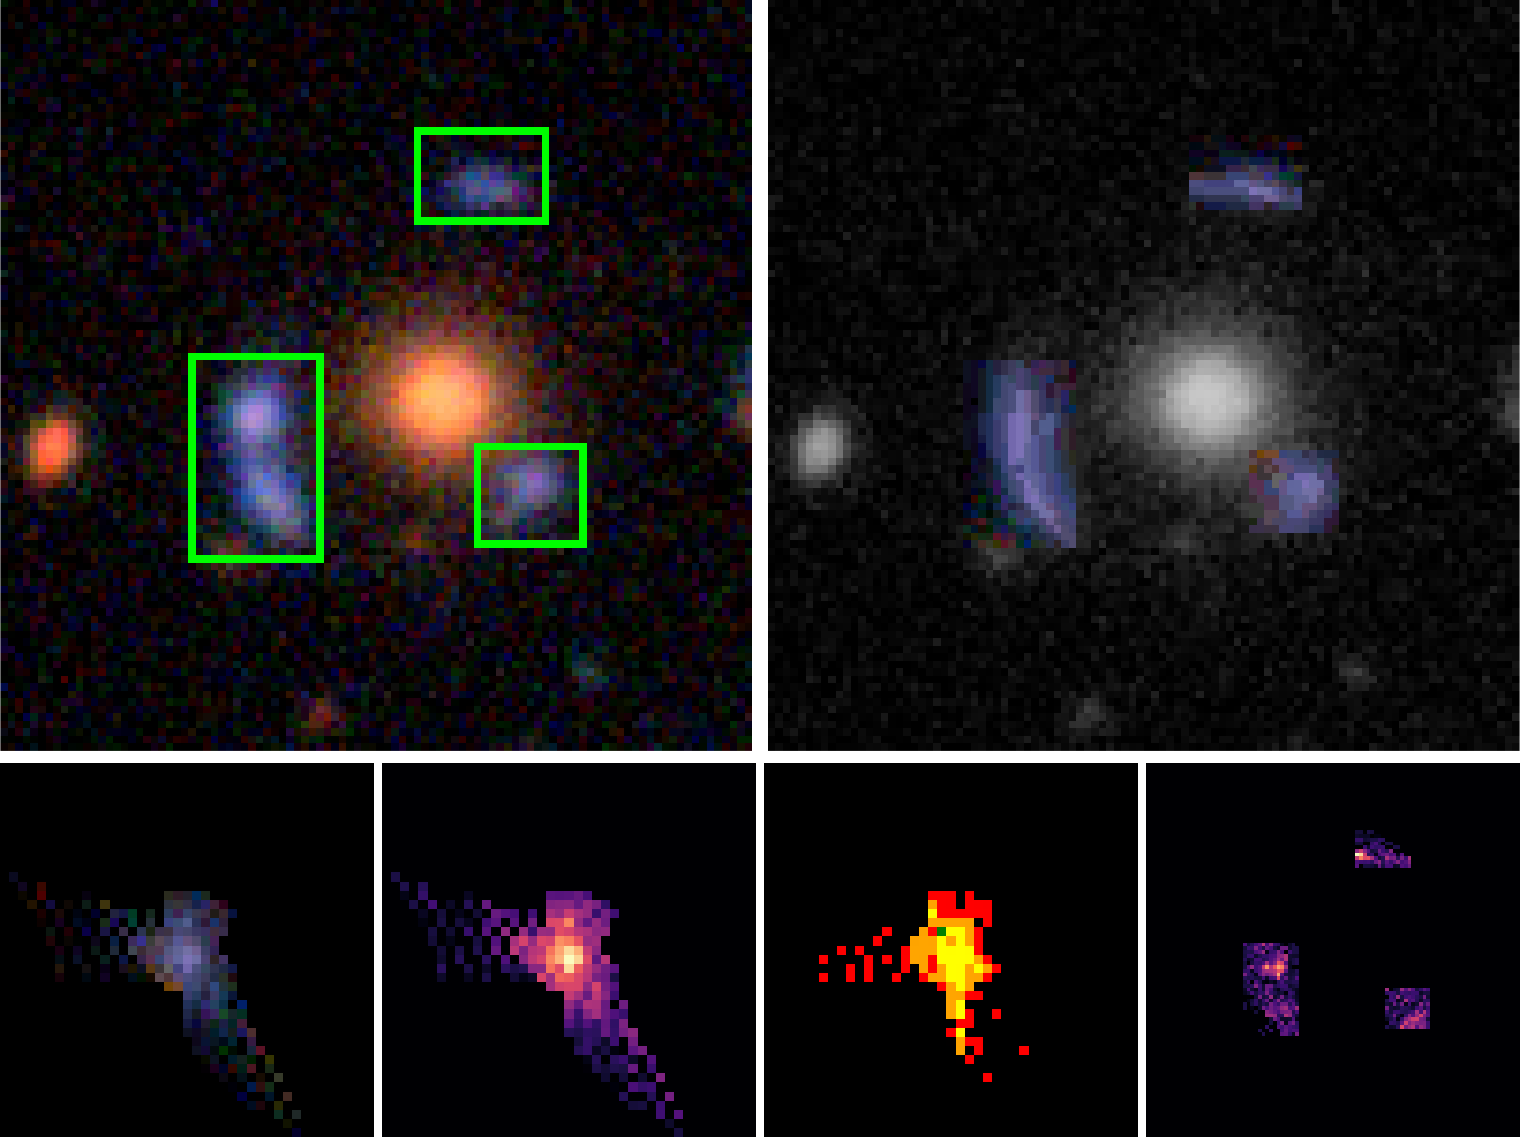
\includegraphics[width=\linewidth]{img/new_synth_img_detailed}
  \caption{Synthetic lensed image with source-profile fitting in SW05
    (J143454.4+522850). Top-left: original image, with areas
    containing lensed images enclosed within green frames.  Top-right:
    synthetic image (coloured arcs) with lensing galaxy and unrelated
    objects in greyscale.  Bottom from left to right: reconstructed
    source in colour, intensity (greyscale), count of lens plane
    pixels per source plane pixel, residual of original image to
    synthetic image.}
  \label{fig:synthimg}
\end{figure}

\begin{figure*}
\includeten{img/nsynth/}{_nsynth}
\caption{}
\end{figure*}


